\documentclass{beamer}

%\usepackage{minted}

\begin{document}

\title[core.logic.intro]{\texttt{core.logic} intro}
\author[e-n@]{Attila Egri-Nagy}
\institute[CRM UWS]{Centre for Research and Mathematics\\School of Computing, Engineering and Mathematics\\ University of Western Sydney}
\date[(nth clj-syd 31)]{clj-syd - The Sydney Clojure User Group, June 25, 2015}

\maketitle

\begin{frame}
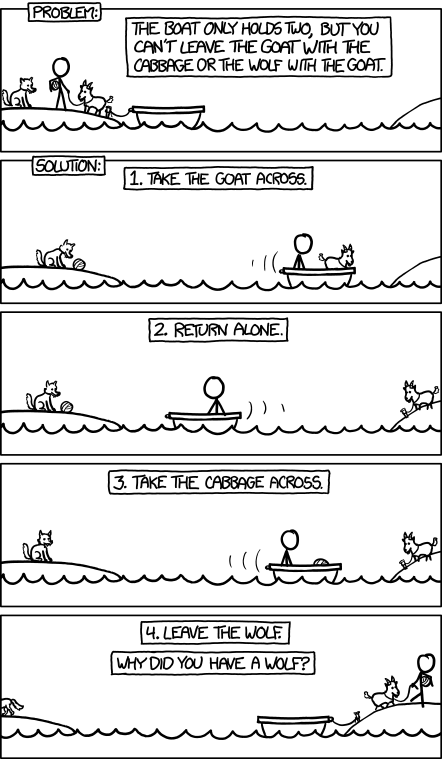
\includegraphics[height=\textheight]{logic_boat.png}
\end{frame}

\begin{frame}\frametitle{What is $x$? What could it be?}
\begin{enumerate}
\item $x$\texttt{=2} \pause\ \ \ \texttt{2, (inc 1)},\ldots\pause
\item \texttt{true} \pause\ \ \ $x$ can be anything\pause
\item \texttt{false} \pause\ \ \ no value of $x$ would satisfy this
  statement\pause
\item $x\in\{1,2,3\}$ and $x\in\{3,4,5\}$ \pause\ \ \ 3\pause
\item \texttt{(cons $x$ (2 3))=(1 2 3)}\pause\ \ \ 1\pause
\end{enumerate}
\end{frame}


\begin{frame}\frametitle{Ways to think about this:}
In order to make the statement \texttt{(cons $x$ (2 3))=(1 2 3)} true,
we need assign the value 1 to $x$.

\begin{itemize}
\item Turning functions into relations. Not just producing output from
  input, but guessing input based on the output.
\item It is a puzzle, statements with holes to fill in.
\item It is a search problem.
\item Assuming we have a set of candidate values, call it a database,
  then it is a database query.
\end{itemize}

\pause
\texttt{core.logic} solves puzzles by search algorithms.
\end{frame}

\begin{frame}\frametitle{Stop talking! Show some code!}
\end{frame}

\begin{frame}\frametitle{Thank You!}
\begin{center}
\huge
\url{https://github.com/egri-nagy}

\url{www.egri-nagy.hu}

\url{replforce.wordpress.com}

\end{center}
\end{frame}


\end{document}

%%% Local Variables:
%%% mode: latex
%%% TeX-master: t
%%% End:
